	\documentclass[a4paper,11pt]{refart}
	\usepackage{listingsutf8}
	%\usepackage[brazilian]{babel}
	\usepackage[utf8]{inputenc}
	\usepackage[T1]{fontenc} % LY1 also works
	\usepackage{tikz}
	\usetikzlibrary{shapes,arrows}
	%% Font settings suggested by fbb documentatio
	\usepackage{float} 
	\usepackage{listings}
	\usepackage{microtype}
	\usepackage{graphicx}
	\usepackage{enumitem}
	\hyphenation{Trans-fe-rên-cias} %Hifenação de palavras
	\setlist{leftmargin=*}
	\lstset{basicstyle=\ttfamily,frame=single,xleftmargin=1em,xrightmargin=1em}
	\usepackage[os=win]{menukeys}
	\renewmenumacro{\keys}[+]{shadowedroundedkeys}
	\usepackage{framed}
	\usepackage{etoolbox}
	\AtBeginEnvironment{leftbar}{\sffamily\small}
	\usepackage[T1]{fontenc}
	\usepackage{lmodern}
	\usepackage{hyperref}
	\usepackage{multirow}                                               
	\usepackage{multicol}                                               
	\usepackage{longtable}
	\usepackage{amsmath,amssymb,mathtools,amsfonts,textcomp}
	\usepackage{dcolumn}
	\usepackage{booktabs}
	\usepackage{makecell}
	\usepackage{tablefootnote}
	\everymath{\displaystyle}
	\hypersetup{colorlinks=true,linkcolor=black,citecolor=blue,urlcolor=blue}

	\renewcommand\theadalign{bc}
	\renewcommand\theadfont{\bfseries}
	\renewcommand\theadgape{\Gape[4pt]}
	\renewcommand\cellgape{\Gape[4pt]}

	\renewcommand\abstractname{}
	\def\CS#1{\texttt{\textbackslash#1}}

	\usepackage[most]{tcolorbox}
	\newtcblisting{commandshell}{colback=black,colupper=green,colframe=black!75!black,
		listing only,listing options={style=tcblatex,language=sh},
		every listing line={\textcolor{red}{\small\ttfamily\bfseries pc@user:\$ }}}

	\usepackage[most]{tcolorbox}
	\newtcblisting{shell}{colback=black,colupper=green,colframe=black!75!black,
		listing only,listing options={style=tcblatex,language=sh},
		every listing line={\textcolor{red}{\small\ttfamily\bfseries}}}

	\title{PRIMoRDiA: User's Guide 1.25v  }
	\author{Igor Barden Grillo \\(\url{barden.igor@gmail.com} )\\\url{github.com/igorChem}}
		
	\begin{document}
	\maketitle
	%***************************************************************
	\begin{abstract}
		\hspace*{-1.4\leftmarginwidth}
		\begin{minipage}{\fullwidth}
			\begin{figure}[H]
				\begin{center}
					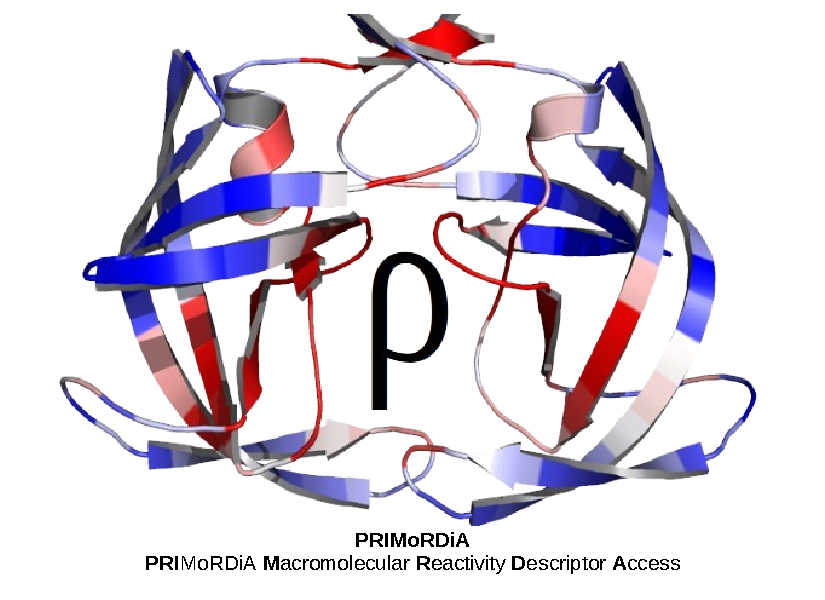
\includegraphics[width=7in]{logo_primordia}
				\end{center}
			\end{figure}
		\end{minipage}
	\end{abstract}
	%***************************************************************
	\newpage
	\tableofcontents
	\newpage

	\section{Introduction}

	PRIMORDIA ( \textbf{PRI}MoRDiA \textbf{M}acromolecular \textbf{R}eactivity \textbf{D}escriptors \textbf{A}ccess ) is a software written in \emph{C++}, developed for post-processing of the results of computational chemistry packages, producing a wide variety of quantum descriptors, which are electronic and reactivity properties of chemical systems.

	PRIMoRDiA implements the main reactivity descriptors of the conceptual DFT Theory, including the mathematical definitions for Fukui's Frontier Electron Orbitals and Pearson's Hard and Soft Acid and Base (HSAB) theories. PRIMoRDiA was developed with a focus on calculating these properties for large molecules that are relevant to biological processes, and therefore there are descriptors modified specifically to meet the particularities of these systems.

	This guide provides general information about the theory behind the descriptors, and details about the usage and interpretation of the results generated by the program. For more information we encourage the contact via the provided emails in the repository and in this document. PRIMoRDiA was developed at the Federal University of Paraíba, at the Laboratory of Quantum and Computational Chemistry.

	This User's Guide is constantly changing. New versions of it will be made available as identified the needs of users and new features being implemented in the program.

	\section{Download and Installation}

	PRIMoRDiA is open source software under the Mozilla 2.0 public license. In the Git Hub repository we provide stable versions of the program, with all source files, test data and binaries already compiled. We strongly recommend compiling the program using \emph{CMake}.

	The program was developed for Linux operational systems, targeting users accustomed to working in the area of molecular modelling. However, for educational and dissemination purposes, code and binary for Windows system is provided in another repository: \url{https://github.com/igorChem/PRIMoRDiA_WIN64}. Remembering that there is no constant support for this version.


	To download the data from the repository you can use the following git command:

	\hspace*{-\leftmarginwidth}
	\begin{minipage}{\fullwidth}
		\begin{commandshell}git clone https://github.com/igorChem/PRIMoRDiA1.0v.git\end{commandshell}
	\end{minipage}

	Through this command, the repository folder will be downloaded in the directory where your terminal is open, and can be easily updated with the command:

	\hspace*{-\leftmarginwidth}
	\begin{minipage}{\fullwidth}
		\begin{commandshell}git pull\end{commandshell}
	\end{minipage}

	Also, on the site itself, it is possible to download a '.zip' containing all the data from the repository.
	However, it is strongly recommended that the user download one of the stable versions, preferably the last one. These stable versions are guaranteed to have all their features properly tested.

	\emph{\textbf{PRIMoRDiA is a program that is under constant development and cloning the repository at any point other than those marked as stable can generate errors in use. }}

	Link to latest version: \url{https://github.com/igorChem/PRIMoRDiA1.0v/releases/tag/v1.25}

	\subsection{CMake Compilation (recommended) }

	Compiling with CMake is very simple to perform, with just a few commands a PRIMoRDiA binary is generated optimized for your machine. The disadvantage of compilation in relation to the use of ready-made binaries is the need to install some libraries required by PRIMoRDiA. Sometimes the user also doesn't have the compilers and CMake itself for the build process.

	On more popular Debian-based Linux distributions, such as Ubuntu and Mint, this can be easily resolved by installing the libraries from the repository.

	By default, PRIMoRDiA uses g++-8 and the Eigen 3 library. To ensure that your machine has what it takes to compile PRIMoRDiA, run the commands below

\hspace*{-\leftmarginwidth}
\begin{minipage}{\fullwidth}
\begin{commandshell}sudo apt install g++-8 
sudo apt install cmake
sudo apt install libeigen3-dev\end{commandshell}
\end{minipage}

	After unzipping the downloaded folder with the stable version, enter the directory and compile it using the following commands:

\hspace*{-\leftmarginwidth}
\begin{minipage}{\fullwidth}
\begin{commandshell}cd /path/to/folder/PRIMoRDiA1.0v
cmake .
make
\end{commandshell}
\end{minipage}

	The compilation process should go smoothly and generate a binary file called "PRIMoRDIA\_1.25v\_LINUX64", if version 1.25 is chosen (most recommended).
	With the command line shown below it is possible to create a shortcut in your ".bashrc" file to run the program from any directory on your system

\hspace*{-\leftmarginwidth}
\begin{minipage}{\fullwidth}
\begin{commandshell}
alias primordia='path/PRIMoRDiA1.0v/PRIMoRDiA\_1.25v\_LINUX64'
\end{commandshell}
\end{minipage}

	\subsection{Compiled Binary}

	In the event that compilation is not possible, the binary for the last stable release is provided in the repository. The same process of putting in the path can be performed. Problems of missing some shared library can happen, as well as the maximum performance not being reached. However, any problems with the execution of the binaries are encouraged to be reported.

	\subsection{Versions}

	As of the release of this User Guide, the program has three stable versions.
	The changes that appear most sensitive to the user are in the input format and in the amount of data extracted by the software. The ideal is always to give preference to the latest stable version.

	\begin{enumerate}
		\item \textbf{1.0v}:\\
		Nine global and fourteen local descriptors implemented. Descriptors for macromolecules, with descriptors individually marked for protein and DNA residues (PDB format).
		\item \textbf{1.2v}:
		\\ New input model, with more control options; R scripts for statistical analysis of reaction trajectory and molecular dynamics, focus on analysis of the reaction coordinate atoms and required input residues. General code tweaks.
		\item \textbf{1.25v}: Three more local hardness methods implemented, and the same local descriptors implemented for volumetric and condensed representation. Adjustments in the automation of results visualization in Pymol. Corrections and standardization of nomenclature.
	\end{enumerate}

	\section{Reactivity Descriptors: Theory}

	Reactivity descriptors (RDs) are theoretical quantities that are convenient for summarizing reactivity properties of molecular systems, as a whole or of different regions and/or atoms. The most successful RDs in the literature are those based on the Conceptual Density Functional Theory (CDFT), which manages to encompass different theories of chemical reactivity through mathematical definitions extracted from the DFT, relating these quantities to well-established chemical concepts\cite{geerlings2003conceptual}.

	These descriptors are obtained from the electronic density calculated from molecular systems, being properties that can only be obtained from quantum calculations. Other electronic properties, such as the electron density itself, total energy and partial charges, are examples of quantities that can be calculated from the electron density and can serve as descriptors. The set of all these properties calculated by PRIMoRDiA are called by our group of Molecular Quantum Descriptors (MQDs) or just Quantum Descriptors.

	The RDs defined within the CDFT come from the total differential equation of the DFT (\autoref{eq.1}) and its derivatives\cite{parr1978elect}, which relates the electronic energy ($E$) with the electron density ($\rho( r)$) of the reference state and the external potential ($\nu(r)$). CDFT RDs can be classified as being global, a number representing an electronic property for the entire system, or local, a function of the system's position.

	\begin{equation}
	dE = \mu dN + \int \rho(r) d \nu (r) dr
	\label{eq.1}
	\end{equation}

	As the main descriptors are derived, the calculation takes place through two approximation methods, which in this case are the Frozen Orbital Approximation (AOC) and the Finite Difference Approximation (FD). Local descriptors can be further separated by the representation/visualization method, Condensed to atoms or into a volumetric representation of a three-dimensional grid, with each voxel represented by a value. This descriptor classification scheme can be viewed in \autoref{fig:M1}.

	\tikzstyle{block} = [rectangle, draw, fill=cyan!20, 
	text width=5em, text centered, rounded corners, minimum height=4em]
	\tikzstyle{decision} = [diamond, draw, fill=yellow!20, 
	text width=4.5em, text badly centered, node distance=3cm, inner sep=0pt]
	\tikzstyle{line} = [draw, -latex']

	\begin{figure}[H]
		\centering
		\begin{tikzpicture}[node distance = 2.5cm, auto]
		\node [block] (init) {CDFT Descriptors};
		\node [decision, below of=init] (typerd) {RD Scope};
		\node [block, right of=typerd] (local) {Local};
		\node [block, left of=typerd] (global) {Global};
		\node [decision, right of=local] (rep) {Vis.};
		\node [block, above of=rep] (cond) {Condensed};
		\node [block, below of=rep] (vol) {3D Grid};
		\node [decision, below of=typerd] (method) {Method};
		\node [block, right of=method] (foa) {FOA};
		\node [block, left of=method] (fd) {DF};
		\path [line] (init) -- (typerd); 
		\path [line] (typerd) -- (local); 
		\path [line] (typerd) -- (global); 
		\path [line] (global) -- (method);
		\path [line] (local) -- (method);
		\path [line] (local) -- (rep);
		\path [line] (method) -- (foa);
		\path [line] (method) -- (fd);
		\path [line] (rep) -- (cond);
		\path [line] (rep) -- (vol);
		\end{tikzpicture}
		\caption{Classification of CDFT Reactivity Descriptors.} \label{fig:M1}
	\end{figure}


	\subsection{Global Descriptors}

	The electronic chemical potential (ECP) is an example of a global reactivity descriptor, which in the DFT is the Lagrangian multiplier (represented by the letter $\mu$) that minimizes the electronic energy in relation to density, given the constant external potential. The table \autoref{tab1} presents the mathematical definition for the global reactivity descriptors and the calculation forms in the two approximation methods.

	\hspace*{-\leftmarginwidth}
	\begin{minipage}{\fullwidth}
		\begin{table}[H]
			\centering	
			\caption{Reactivity Descriptors implemented in PRIMoRDiA}
			\begin{tabular}{c|c|c|c|c}
				\toprule
				DR global & Definition in CDFT  & FOA & FD & Ref. \\
				\midrule
				IP & - & $- E_{HOMO}$ & $E_{N-1}-E_{N}$ & \\  \hline	
				EA & - & $- E_{LUMO}$ & $E_{N}-E_{N+1}$ & \\ \hline	
				$\mu$  & $\left(\frac{\partial E}{\partial N} \right)_\nu$  & $\frac{E_{HOMO} + E_{LUMO}}{2}$ &$\frac{E_{N-1}-E_{N+1}}{2}$ & \cite{ribeiro2017atlas}\\ \hline			
				$\eta$  & $\left(\frac{\partial ^2  E}{\partial N ^2} \right)_\nu$ &$E_{LUMO} - E_{HOMO}$ &$E_{N-1}+E_{N+1}-2E_{N}$ & \cite{parr1983absolute}\\ \hline
				Softness($S$)  & $1/\eta$  & - & -  & \cite{parr1983absolute} \\ \hline
				$\omega$  & $\frac{\mu^2S}{2}$  &-  &-  & \cite{cedillo2012local} \\ \hline
				$nMax$  & $-\frac{\omega}{\eta} $ & - & - & \cite{cedillo2012local}  \\ 
				\bottomrule
			\end{tabular} 
			\label{tab1}	
		\end{table}	
	\end{minipage}

	The ECP establishes the propensity of the system to donate electrons, and when the values between different molecular system are equal, the transfer of electrons ceases, characterizing the equilibrium state\cite{parr1983absolute}. This is why $\mu$ is named in analogy to the molar chemical potential of classical thermodynamics.

	The principle of Hard and Soft Acids and Bases (\textit{HSAB: Hard and Soft Acid and Base}) by Pearson\cite{pearson1987recent} is one of the theories of chemical reactivity that gained theoretical and mathematical foundations within the CDFT. Pearson created concepts called chemical hardness and softness to explain the affinity between acids and bases by the Lewis model, based on the observation of atomic and molecular characteristics and the reactivity series\cite{Pearson1963}. From this study, it was defined that Hard acids are small and poorly polarizable electron acceptors, which in turn tend to chemically interact with hard bases, which are electron donors with the same volume and polarizability characteristics. This interaction between species considered chemically "hard" by Pearson occurs through interactions controlled by charge, forming bonds of ionic character.

	On the other hand, soft acids and bases are polarizable and bulky species, where the interaction is governed by the delocalization of the boundary molecular orbitals, with a donation of electrons from the higher-energy occupied orbital (HOMO) of the base to the acid lower-energy virtual orbital (LUMO). In this process of interaction of soft species, there is a net charge transfer from the base to the acid and there is also a greater chance of forming bonds with a covalent character. Therefore, it is possible to establish complementary rules to understand the main forces that lead a chemical reaction to happen using this Pearson principle.

	However, until the consolidation of the CDFT, the HSAB was a theory without mathematical support and a systematic way of determining scalar hardness and softness. In CDFT, hardness is primarily seen as a property of the system that represents its resistance to donate electrons, being also a characteristic of poorly polarizable and small-volume systems, that is, where electrons are more agglutinated to the nuclei.

	The mathematical definition of the global descriptor associated with chemical hardness in CDFT is the derivative of ECP with respect to the number of electrons, the same as the second derivative of energy with respect to the number of electrons, and commonly represented with the Greek letter $\eta$ . Briefly, global chemical softness is defined as the reciprocal of hardness, usually represented by the letter $S$.

	Other global descriptors that can be obtained in CDFT are basically about these charge transfer processes, which are generally used to rationalize chemical reactions. For example: The maximum number of electrons that can be received by a system by an ideal donor $nMax$; the stabilization of energy when the system receives this number of electrons, which can be called electrophilicity and represented in the CDFT literature with the Greek letter $\omega$\cite{Pearson1990}.

	\subsection{Calculation Methods}

	As already mentioned above, most reactivity descriptors are derived from energy and/or electron density with respect to the number of electrons. The number of electrons is always integer, and therefore there is no continuous function of this quantity, being necessary that these derivatives are approximated through mathematical methods.

	The most common method for numerically determining derivatives, whatever it is, is the finite difference (FD) method. For the CDFT quantities, the calculations have to be performed using data from the electronic structure of three states of charge of the system. For global descriptors, the information needed is the electronic energies of these three states of charge, the reference state, positively charged (at least one electron less) and negatively charged (at least one electron more).

	For the local descriptors this logic applies in the same way to the electron density, or partial charge in the case of the representation condensed by atoms. All electronic structure calculations must be performed for the same atomic coordinates of the reference state, that is, for the same position of the nuclei, respecting the condition of constant external potential required by these derivatives.

	The other method of calculation is called the Frozen Orbital Approximation (\textit{Frozen Orbital Approximation})\cite{yang1984electron}, which uses the information from the boundary molecular orbitals, HOMO and LUMO, and disregards the change in energy/spatial distribution of the inner orbitals, which justifies the name of the method.

	For global descriptors in particular, the calculations are performed with the energy of the molecular orbitals HOMO and LUMO, and it is also known as Koopmans' Theorem\cite{manne1970koopmans}, which states that the energy of HOMO is the approximation of the Ionization Potential (IP) and the LUMO energy as the approximation of Electronic Affinity (EA). The big difference between this approach and the finite difference one is that it only requires an evaluation of electronic structure (commonly called \textit{Single Point} in English). And in relation to the local descriptors, obtaining the probability densities of these orbitals requires a negligible computational effort in comparison with which is necessary for the total electronic density.

	Therefore, FOA has a significantly lower computational cost than FD, the latter being prohibitive for large molecules. As for accuracy, the approximation of FD by definition is theoretically greater, since it considers the perturbation of the entire electronic density when the system participates in charge transfer processes. However, the FOA is estimated by molecular orbitals that generally have great importance in explaining the chemical reactivity of molecules, as it gives the probability distribution of the location of electrons that are more susceptible to chemical processes.

	\subsection{Local Descriptors}

	The mathematical definition of a local descriptor is a function of the three-dimensional space $r$, that is, given a point in space, the descriptor takes on a certain value. The electron density $\rho$ is one of those local quantities by definition, where the density value is defined by the product of the occupied molecular orbitals $\phi_{occ}(r)$ (\autoref{eq.2}), which by in turn are linear combinations of atomic orbitals $\phi $, where the coefficients $c_i$ are determined by computational chemistry methods.

	\begin{equation}
	\rho(r) = \sum_{i}^{occ} |\psi(r)^2_i|
	\label{eq.2} 
	\end{equation}

	\begin{equation}
	\psi(r)_i = \sum_{i} c_i \phi(r)
	\label{eq.3} 
	\end{equation}

	\subsubsection{Representation Methods}

	The practical way to represent these local descriptors is to define a three-dimensional grid, where each point $r$ relates three-dimensional coordinates of the chemical system with a value. These dots are known as \textit{voxel}, the three-dimensional analogue of the pixel, and are usually collected in a formatted file called \textit{Gaussian Cube}, or simply cube, with the extension ".cube". This file has a pattern that is recognized by the vast majority of molecular visualization software, being able from them to create graphic representations of iso-surfaces, render more than one of these iso-surfaces assigning different colors and opacities, which results in a volumetric representation.

	Within the language of quantum descriptors adopted by PRIMoRDiA, this representation is known as volumetric. PRIMoRDiA calculates 21 electronic properties/reactivity descriptors that can be written to disk as formatted Cube files. For this, it is necessary for the user to define the non-zero resolution of the three-dimensional grid and provide the electronic structure data necessary for the calculation of these quantum descriptors. More details on the parameters, input and the descriptors themselves are given in the next sections of this guide.

	As stated before, each voxel represents a local descriptor value for a given point $r$. To facilitate the chemical interpretation and numerical manipulation of these properties it is possible to integrate them into a common base $\Omega$. 

	For example, a fraction of the electron density can be attributed to an atom of the molecular system through a population analysis, such as that of Muliken or Lowdin for example. 

	These numerical methods sum the coefficients of molecular orbitals, or density matrix elements, that are assigned to atomic orbitals, partitioning these values for each atom. This process is known as condensation, generating a condensed representation for atoms, and often shortened to just 'condensed'. In the generic case shown in \autoref{eq.4}, the descriptor $f(r)$ can have its part assigned to the atom $k$ through the integration of the values of $f(r)$ in the base functions referring to this one atom.

	PRIMoRDiA calculates the descriptors and writes a file with the list of values of the local descriptors ordered by the atom index in the file provided to the software.

	\begin{equation}
	f_k^{a} = \int_{\Omega k} f(r)dr
	\label{eq.4}
	\end{equation} 

	\subsubsection{Fukui Functions} 

	The Fukui function can be considered the first local reactivity descriptor, defined in the CDFT as the derivative of the electron density with respect to the variation in the number of electrons (\autoref{eq.5}), being required in the calculation of most other descriptors locations. There are other earlier local descriptors, such as the very delocalizability of boundary orbitals created by Kenichi Fukui that inspired the CDFT\cite{fukui1970theory} Fukui function and indices. However, these other properties had their concepts consolidated in the CDFT through a mathematical tool, making these other quantities obsolete.

	As far as reactivity is concerned, the Fukui function indicates the places where the electron density is most likely to vary when the system participates in a charge transfer process. For the reasons already mentioned, the descriptors that are derived with respect to the number of electrons must be approximated by some method. 

	\begin{equation}
	f(r) = \left(\frac{\partial \rho(r)}{\partial N} \right)_\nu
	\label{eq.5}
	\end{equation}

	The Fukui indices arise from the approximation of the Fukui function by the finite difference method, where the derivative is approximated by the left and right limits in relation to the variation in the number of electrons $N$. The left approximation assumes a value less than $N$, the minimum possible being $N-1$ and the value of the density in the reference state. The difference between the reference state and the positively charged state corresponds to the Fukui index that describes the local susceptibility of the system to receive an electrophilic attack, signaled as $f^{-}(r)$ as shown in \autoref{eq.6}.

	\begin{equation}
	f^{-}(r) = \rho(r)_{N} -\rho(r)_{N-1}
	\label{eq.6}
	\end{equation}

	The interpretation of the $f^{-}(r)$ calculation is that the difference in electron density between these different states of charge will reveal the regions where electron density is left over when the system loses an electron. This excess electron density is the most likely to "detach" from the system and serve to form a bond with an electrophile or be transferred.

	The right approximation considers a state of charge with a number of electrons greater than $N$, being at least $N+1$. The difference between the negatively charged and reference state of charge is the local susceptibility index of the system to receive a nucleophilic attack, represented by $f^{+}(r)$ shown in \autoref{eq.7}.

	\begin{equation}
	f^{+}(r) = \rho(r)_{N+1} -\rho(r)_{N}
	\label{eq.7}
	\end{equation}

	The interpretation of the $f^{+}(r)$ calculation is that the difference in electron density between these different states of charge will reveal the regions where the electron density is concentrated when the system gains an electron, indicating the most likely region where a nucleophile will form a bond or transfer electron density.

	The average value of these two indices is the derivative at point 0, and is used to indicate the local susceptibility of the system to receiving a radical attack. What in practice is observed in the equation of this index is the average reactivity between the susceptibility to a nucleophilic attack and an electrophilic attack, that is, the average reactivity of the system regardless of the type of attack.

	\begin{equation}
	f^{0}(r) = \frac{\rho(r)_{N+1} -\rho (r)_{N-1}}{2}
	\label{eq.8}
	\end{equation}

	These descriptors have some English names and terms that may vary. This is as a matter of balance between precision of terms and their chemical understanding. As for example the \textit{susceptibility to electrophilic attack} which is nothing more than the local nucleophilicity of the system. The former is the more technical term referring to what was calculated and the latter has a greater commitment to understanding the theoretical quantity in question.

	This is important to say because different versions of the program and published works of our group adopt different nomenclatures for these local descriptors, which over time has been increasingly considered the transparency and simplification of the nomenclature than its precision in relation to what is defined mathematically. This is all detailed in the next section of the user guide. As well as ''indexes'' and ''local functions'' are similar and will be invoked depending on the authors' choice.

	A fourth Fukui index that can be considered is the Dual Fukui index or just the Dual descriptor, which has this name because it simultaneously indicates the sites of the system susceptible to electrophilic and nucleophilic attacks. The dual descriptor $\Delta f^{\pm}$ is calculated by the difference $f^{+}(r)$ and $f^{-}(r)$ ( \autoref{eq.9}), that is , the effective local reactivity of the system. Also, this descriptor is indicated to be sometimes more accurate than $f^{+}(r)$ and $f^{-}(r)$ individually due to the error cancellation that eventually occurs when there is a subtraction between these quantities\cite{martinez2015dual}. In PRIMoRDiA, we adopted the name ''Netphilicity'', in place of the dual descriptor.

	\begin{equation}
	\Delta f^{\pm}(r) = f^{+}(r) - f^{-}(r)
	\label{eq.9}
	\end{equation}

	Fukui functions can also be obtained with the frozen orbital approximation, which assumes that the infinitesimal variation in the number of electrons in the system causes an irrelevant change in the inner molecular orbitals. In the case of $f^{-}(r)$ its calculus definition as a function of the density of the $M$ energy levels (molecular orbitals/Khon-Sham orbitals) is given in \autoref{eq.10} and the approximation turns out to be the density of the highest-energy occupied boundary molecular orbital, aka HOMO (\autoref{eq.11}).

	\begin{equation}
	f^{-}(r) = \lim_{\delta \to 0^-} \frac{\partial \rho_{M+\delta}(r)}{\partial N} = |\phi_{M}(r)|^2  +\sum_{i=1}^{M-1} \frac{\partial}{\partial N} |\phi_i(r)|^2
	\label{eq.10}
	\end{equation}

	\begin{equation}
	f^{-}(r) = |\phi_{HOMO}(r)|^2 
	\label{eq.11}
	\end{equation}

	For $f^{+}(r)$ it is very similar, where the derivative is taken from the limit of a positive (right) change in the number of electrons(\autoref{eq.12}), resulting in the energy level $ M+1$, which is the lowest energy virtual energy level, aka LUMO (\autoref{eq.13}).

	\begin{equation}
	f^{+}(r) = \lim_{\delta \to 0^+} \frac{\partial \rho_{M+\delta}(r)}{\partial N}	 =  |\phi_{M+1}(r)|^2  + \sum_{i=1}^{M} \frac{\partial}{\partial N} |\phi_i(r)|^2
	\label{eq.12}
	\end{equation}

	\begin{equation}
	f^{+}(r) = |\phi_{LUMO}(r)|^2 
	\label{eq.13}
	\end{equation}

	For the calculation of $f^{0}(r)$ by the FOA, it is done by the average between $f^{+}(r)$ and $f^{-}(r)$, or following the logic of using the boundary molecular orbitals, $f^{0}(r)$ can be approximated by the uniquely occupied molecular orbital, abbreviated in English as SOMO (Single Occupied Molecular Orbital) (\autoref{eq.14}).

	\begin{equation}
	f^{0}(r) = |\phi_{SOMO}(r)|^2 
	\label{eq.14}
	\end{equation}

	Fukui functions/indices can still be represented in condensed form for atoms for each of the possible approximations. In the case of finite differences, the electron density at point $r$ is replaced by the partial charge of each atom, which will depend on the population analysis used. The function $f^{-}$ is defined for each atom $k$ as shown in \autoref{eq.15} and $f^{+}$ in \autoref{eq.16}. Consequently, $f^{0}(k)$ taken as the average of $f^{+}_k$ and $f^{-}(k)$, and $\Delta f^{\pm}$ as the difference.

	\begin{equation}
	f^{-}(k) = q_{k [N]} - q_{k [N-1]}
	\label{eq.15}
	\end{equation}

	\begin{equation}
	f^{+}(k) = q_{k [N+1]} - q_{k [N]}
	\label{eq.16}
	\end{equation}

	For the FOA, it is the boundary orbitals that must be condensed for the atoms, and this is done in order to partition these molecular orbitals by the contribution of the AO atomic orbitals of index $\nu$ and their overlap with the other orbitals ($\ mu$) of the same atom $k$ counting as the cross product weighted by the overlap matrix, also called the one-electron integrals $S_{\nu\mu}$. This process can be performed for the probability density condensation for any molecular orbital $\psi^i$, as shown in \autoref{eq.31}.

	For FOA, condensation by atoms is performed using the probability density of the boundary orbitals, whose contribution is given by the coefficients of the AO atomic orbitals with index $\nu$ and their overlap with the other orbitals ($\mu$) of the same atom $k$ counting as the cross product weighted by the overlap matrix, also called the one-electron integrals $S_{\nu\mu}$. This process can be performed for the probability density condensation for any molecular orbital $\psi^i$, as shown in \autoref{eq.17}.

	\begin{equation}
	|\psi^i(k)|^2  =\sum_{\nu \in k}^{AO} \Bigg \{ |C_{\nu i}|^{2} + \sum_{\mu \notin \nu }^{AO} |C_{\nu i} C_{\mu i}|S_{\mu \nu} \Bigg \}
	\label{eq.17}
	\end{equation}

	Therefore, for $f^-(k)$ the probability density of HOMO ( \autoref{eq.18} ) is used and for $f^+(k)$ the LUMO ( \autoref{eq.18} ).

	\begin{equation}
	f^-(k) =|\psi^{HOMO}(k)|^2 =  \sum_{\nu \in k}^{AO} \Bigg \{ |C_{\nu HOMO}|^{2} + \sum_{\mu \notin \nu }^{AO} |C_{\nu HOMO} C_{\mu HOMO}|S_{\mu \nu} \Bigg \}
	\label{eq.18}
	\end{equation}

	\begin{equation}
	f^+(k) = |\psi^{LUMO}(k)|^2 = \sum_{\nu \in k}^{AO} \Bigg \{ |C_{\nu LUMO}|^{2} + \sum_{\mu \notin \nu }^{AO} |C_{\nu LUMO} C_{\mu LUMO}|S_{\mu \nu} \Bigg \}
	\label{eq.19}
	\end{equation}

	So far we have defined the forms of calculation for the Fukui functions, in their condensed and volumetric form, and for the two types of possible approximation.

	\subsubsection{Local Softness and Electrophilicity}

	Global descriptors can be defined locally by replacing the number of electrons with the electron density, which in fact is the local representation of the number of electrons. A classic example is the local softness $s(r)$, defined in \autoref{eq.20} as the derivative of the electron density with respect to the chemical potential with constant external potential. By Maxwell's relations also shown in \autoref{eq.20}, this definition can be obtained by the global softness product and the Fukui function. Thus, the local softness is the global softness distributed to the regions of greater reactivity of the system, being a combination of a global and a local descriptor\cite{Lee1988}.

	\begin{equation}
	s(r)= \left(\frac{\partial \rho(r)}{\partial \mu} \right)_\nu =
	\left(\frac{\partial N}{\partial \mu}\right)_\nu
	\left(\frac{\partial \rho(r)}{\partial N} \right)_\nu = Sf(r)
	\label{eq.20}
	\end{equation}

	As the Fukui function is divided into different indices in the calculation methods in relation to the type of attack that the system can suffer, the local softness calculation ends up suffering the same partition, obtaining the forms described in \autoref{eq.21}--\autoref{eq.24}.

	\begin{equation}
	s^-(r) = Sf^-(r)
	\label{eq.21}
	\end{equation}

	\begin{equation}
	s^-(r) = Sf^-(r)
	\label{eq.22}
	\end{equation}

	\begin{equation}
	s^{0}(r) = Sf^{0}(r)
	\label{eq.23}
	\end{equation}

	\begin{equation}
	s^{\pm}(r) = Sf^{\pm}(r)
	\label{eq.24}
	\end{equation}

	Also, there is the hyper-softness, which is the derivative of the local softness with respect to the number of electrons, replacing the Fukui function by the dual descriptor $f^{\pm}(r)$ and the global softness by its square\cite {sandoval2018theoretical}. The main advantage of this descriptor is that it can be used to simultaneously assess local softness in electrophilic and nucleophilic regions.

	\begin{equation}
	s^{2}(r) = S^2f^{\pm}(r)
	\label{eq.25}
	\end{equation}

	The local electrophilicity arises in the same way as the local softness, and can be calculated as the product of the total electrophilicity by the Fukui functions\cite{noorizadeh2013evaluation}, as shown in \autoref{eq.26}. Soon the same effect of division by type of attack also presents itself. Local electrophilicity partitions the global referent property which is the stabilization of electronic energy given in the process of receiving electrons by the system. Therefore, the default definition is given using $f^+(r)$, which describes the locations most prone to electrophilic attacks. When using the dual descriptor $f^{\pm}(r)$ instead of $f^+(r)$, the multiphilic descriptor $\Delta \omega(r)$ appears, which serves to describe the same type of process regardless of the attack type\cite{padmanabhan2007multiphilic}.

	\begin{equation}
	\omega(r) = \omega f^+(r)
	\label{eq.26}
	\end{equation}

	\begin{equation}
	\Delta \omega(r) = \omega f^{\pm}(r)
	\label{eq.27}
	\end{equation}

	By the mathematical definition these descriptors contain redundant local information in relation to the Fukui functions, since they will indicate as more reactive regions where thw values of Fukui index is at maximum. However, the combination of information from the global descriptors allows a comparison of local reactivity for different molecules, since the Fukui functions are normalized and are not able to say whether a certain atom $\alpha$ in molecule A is more reactive than the atom $\beta$ belonging to the molecule B\cite{Roy1998}. Fukui functions represent intramolecular reactivity, and local descriptors such as local softness and local electrophilicity can be used for a comparison of local intermolecular reactivity.

	The global descriptors serve for a comparison of reactivity between different molecular systems, yielding an intermolecular analysis, the sites for a comparison of reactivity by region of the molecule, and when the two are combined it is possible to compare the reactivity of regions of different molecules, that is, a local intermolecular comparison.

	\subsection{Local Hardness Methods}

	Through the development of reactivity theories, Klopman and Fukui summarized the forces that govern chemical processes into two types: Orbital-Controlled and Charge-Controlled\cite{klopman1968,fukui1970theory}. Pearson defined that Controlled-by-Load processes are carried out by hard acids and bases, thus being hard-hard interactions, and Controlled-by-Orbital processes are therefore soft-soft\cite{Pearson1990}.

	The first has the approximation of species governed by Coulomb forces, resulting in bonds of greater ionic character than covalent. On the other hand, the mole-mole interactions are characterized by a significant charge transfer, and overlapping molecular orbitals on the boundary, resulting in bonds of a more covalent than ionic character.

	We have seen that there is a definition of local softness and naturally it is expected that there is local hardness. In fact, if we take the reciprocal of \autoref{eq.20} we get the definition shown in \autoref{eq.28}, a valid derivative in CDFT. However, the integration of $\eta(r)$ does not result in the global quantity without multiplication by a kernel function, as shown in \autoref{eq.29}. This introduces an ambiguity in the condition of the local descriptor, which when integrated into the entire space $r$, should fully represent the global quantity.

	\begin{equation}
	\eta(r) = \left( \frac{\partial \mu}{\partial \rho(r) } \right)_\nu
	\label{eq.28}
	\end{equation}

	\begin{equation}
	\eta = \int \eta(r) f(r)
	\label{eq.29}
	\end{equation}

	The CDFT is a very rigorous area in terms of its mathematical foundation and since its definition, local hardness has been the subject of debates and developments, with currents of researchers seeking a mathematical definition that respects the condition of integration and another current seeking its effectiveness in the description of the regioselectivity of charge-controlled reactions. From this "local hardness problem", several "working equations" emerged, which are mathematical definitions for the calculation of this property for its application.

	In order to make available all possible tools for calculating properties derived from the electronic structure of macromolecules, PRIMoRDiA has implemented the most widespread working equations in the literature so that the user can decide which is the most appropriate for his object of study. In version 1.0v the software is released with four local hardness versions. In the latest stable version corresponding to this user guide (1.25v), some local hardness variations were implemented and some more local electronic properties were made available that can be used to study hard-hard processes. The complete list of these quantities is presented in the later section of this guide.

	As this section of the user guide is about the basic theory of quantum descriptors, some important deductions from these working equations, the origin of their approximations and what they can represent in the interpretation of the reactivity of chemical systems will be demonstrated.

	\subsubsection{Thomas-Fermi-Dirac Approximation}

	The first working equation arises as soon as the partial derivative shown in \autoref{eq.28} was defined by Berkowitz in 1985\cite{berkowitz1985concept}, as a function of the Electronic energy functional $F[\rho]$ through the relation shown in \autoref{eq.29}. The local hardness is a quantity proportional to the integral of the product between the electron density and the second derivative of the total electronic energy functional with respect to the electron density. When a property is already derivative with respect to $\rho(r)$, the application of another derivative with respect to electron density will be with respect to a $r'$ representing a point in three-dimensional space other than $r $.

	\begin{equation}
	\eta(r) = \left( \frac{\partial \mu}{\partial \rho(r) } \right)_\nu = \frac{1}{2N} \int \frac{\delta^2 F[\rho]}{\delta \rho(r) \delta \rho(r')} \rho(r')dr'
	\label{eq.30}
	\end{equation}

	This definition arises from the relationship that exists between the total energy functional $E[\rho]$ and $F[\rho]$, given in \autoref{eq.31}, where the contribution due to the potential of the nuclei of the atoms $v(r)$ of the electronic part. In turn, $F[\rho]$ is divided into three independent electronic contributions: kinetic energy functional $T[\rho]$; classical coulomb interaction functional $J[\rho]$; and the electronic exchange-correlation functional $E_{xc}[\rho]$ (\autoref{eq.32}). Therefore, the local hardness can also be divided into three, each corresponding to an electronic energy functional that composes $F[\rho]$ (\autoref{eq.33}).

	\begin{equation}
	E[\rho] = \int \rho(r) d \nu (r) dr + F[\rho]
	\label{eq.31}
	\end{equation}

	\begin{equation}
	F[\rho] = T[\rho] + J[\rho] + E_{xc}[\rho]
	\label{eq.32}
	\end{equation}

	\begin{equation}
	\eta_{F} (r) = \eta_{T}(r)+ \eta_{J}(r) - \eta_{K}(r)
	\label{eq.33}
	\end{equation}

	In the Thomas-Fermi-Dirac (TFD) model for these functionals, the local hardness referring to the kinetic energy functional and the exchange-correlation functional can be neglected, since these same functionals assume negligible values in these regions of the chemical systems where the reactions, so that \autoref{eq.30} can be approximated only using the classical electron-electron interaction functional, as shown in \autoref{eq.34}. 

	This approximation greatly facilitates the definition of a first working equation for local hardness, since the derivative of $J[\rho]$ (\autoref{eq.35})  with the respect to electron density is trivial and the calculation of $\eta(r)$ is as shown in \autoref{eq.36}

	\begin{equation}
	\eta^{TFD} (r) = \frac{1}{2N} \int \frac{\delta^2 J[\rho]}{\delta \rho(r) \delta \rho(r')} \rho(r')dr'
	\label{eq.34}
	\end{equation}

	\begin{equation}
	J[\rho] = \frac{1}{2} \int \int \frac{\rho(r) \rho(r')}{|r-r'|} dr dr'
	\label{eq.35}
	\end{equation}

	\begin{equation}
	\eta^{TFD} (r) = \frac{1}{2N} \int \frac{\rho(r')}{|r-r'|} dr'
	\label{eq.36}
	\end{equation}

	This is the first working equation for local hardness, used until today, and can be found with the "TFD", indicating the approximation of the explained model. Therefore, the local hardness can be estimated as the integral of the electronic density in the positions $r'$ of the system, which are all other than the $r$ which is the position for which the property is being calculated. The quantity is still normalized by the number of electrons $N$, but its integral still does not correspond to the global quantity, by the very definition of the derivative. In PRIMoRDiA, both this approximation and the full estimate of $\eta(r)$ with the other two functionals are available.

	For condensation for atoms, the electron density is calculated for each atom using the sum of the product of the molecular orbitals, and the coordinates of the nuclei substituting the values of $r$ and $r'$.

	\subsubsection{Fukui Potential}

	A work equation that came soon after was the one that approximates the electron density in \autoref{eq.36} by the Fukui function, while removing the normalization factor in relation to the number of electrons by the fact of the Fukui function already normalized, resulting in \autoref{eq.37}. This descriptor is also known as the Fukui potential, for $r = 0$ it is considered the hardness at the position of the nucleus of the atom, since its definition is also equivalent to the hardness derivative with respect to the variation of the external potential. Furthermore, this approximation is justified by the fact that the Fukui function is considered to represent the most reactive portion of the electron density, which in theory would increase the predictive power of the reactivity of the system.

	\begin{equation}
	\eta^f(r) = \int \frac{f^{-}(r')}{|r - r'|}
	\label{eq.37}
	\end{equation}

	As the Fukui potential depends on the calculation of Fukui functions, this descriptor is divided into three and the calculation methods depend on the approximation. Therefore, the first Fukui potential that we define using $f^-(r)$ is the left Fukui potential $\eta^{f^-}(r)$ which is implemented in PRIMoRDiA together with the Fukui potential to the right $\eta^{f^+}(r)$ and average Fukui potential $\eta^{f^0}(r)$. In the Frozen Orbital approximation these descriptors depend on regions where there is greater interaction with the density of the boundary orbitals, and the results end up being quite different when it is done with finite differences. The great computational advantage in this descriptor is that in AOC the calculation is significantly faster than the first work equation presented, which requires the calculation of the total electron density.

	\subsubsection{Local Chemical Approximation Potential}

	The third working equation arises from an attempt to resolve the ambiguity of the local hardness definition by developing a local version of the electronic chemical potential. This is because the derivative of the local PQE with respect to the number of electrons is a valid definition for local hardness (\autoref{eq.38}), and its integral would give the derivative of the global PQE $\mu$ with respect to the number of electrons , which is the global hardness itself, as shown in \autoref{eq.39}.

	\begin{equation}
	\eta(r) = \left( \frac{\partial \mu(r)}{\partial N } \right)_\nu
	\label{eq.38}
	\end{equation}

	\begin{equation}
	\eta = \int \left( \frac{\partial \mu(r)}{\partial N } \right)_\nu dr = \left( \frac{\partial \mu}{\partial N } \right )_\nu
	\label{eq.39}
	\end{equation}

	The major theoretical issue in this case is that the PQE is a descriptor that indicates the chemical equilibrium of the system in relation to its variation in the number of electrons, and the system in equilibrium would not present a tendency towards an internal transfer of electrons from one region to another. . This is what we actually define as a global descriptor, showing that the value is identical in all regions of the system and therefore it is in equilibrium.

	Even so, a mathematical definition for the PQE derivative with respect to the number of electrons for a given $r$ was developed as a mathematical device to arrive at a valid definition of local hardness that is integrable for the global property. For this, Gal and collaborators used mathematical relations intrinsic to the normalizable functionals\cite{gal2011new}, making the derivative of the total electronic energy functional $E_[\rho]$ with respect to the electron density to be written as in \autoref {eq.40}.


	\begin{equation}
	\frac{\delta E[\rho]}{\delta \rho(r)} = \frac{1}{N} \int \rho(r') \frac{\delta E[\rho]}{\ delta \rho(r')} dr'
	\label{eq.40}
	\end{equation}

	The electronic chemical potential ends up being written as an integral over the space of another local quantity, in this case the electron density, as shown in \autoref{eq.41}. Therefore, removing the integral in \autoref{eq.41}, the PQE becomes a function of $r$, that is, a local function, which can be written as in \autoref{eq.42}.

	\emph{Basically the local PQE is the local quantity distributed by the normalized electron density, and therefore seamlessly integrating into the global quantity}.


	\begin{equation}
	\mu = \frac{1}{N} \int \rho(r) \frac{\delta E[\rho]}{\delta \rho(r)} dr
	\label{eq.41}
	\end{equation}

	\begin{equation}
	\mu(r) = \frac{\rho(r)}{N} \frac{\delta E[\rho]}{\delta \rho(r)} dr' = \frac{\rho(r)} {N} \mu
	\label{eq.42}
	\end{equation}

	From this definition of $\mu(r)$, it is possible to write the derivative of the local PQE with respect to the number of electrons resulting in the local hardness $\eta(r)$, as another working equation shown in \autoref{ eq.43}. In the first part of the equation, the local part is given by the difference between the density of HOMO and the normalized electron density, whose integral is zero. In the second part, the integral equals the global hardness, resolving the ambiguity of the local hardness definition.

	\begin{equation}
	\eta(r) = \left (\rho(HOMO) - \frac{\rho(r)}{N} \right) \frac{\mu}{2N} + \frac{\rho(r)}{N}\eta
	\label{eq.43}
	\end{equation}

	\subsubsection{Fukui Distribution}

	The last development of the working equation discussed here is the one that distributes the global hardness using the left Fukui functions $f^-(r)$ and the right $f^+(r)$. In this case, the global hardness is the difference in its Ionization Potential and Electronic Affinity (\autoref{eq.44}) plots, and the local hardness is defined as the product difference between PI and $f^-(r)$ and from the product enter EA and $f(r)^+$ (\autoref{eq.45}).

	\begin{equation}
	\eta = PI - AE
	\label{eq.44}
	\end{equation}

	\begin{equation}
	\eta(r) = PI f^-(r) - AE f^+(r)
	\label{eq.45}
	\end{equation}

	This working equation was proposed by Meneses et al.\cite{meneses2004proposal}, and is based on the notion that electrophilic species have high PI and a nucleophile would have a low EA, maximizing $\eta(r)$ where the Fukui functions on the left indicate the most reactive electron density. Despite being based on well-established chemical reactivity concepts and complying with the integration requirement for global quantity, this working equation depends heavily on properties that correlate with mole-mole interactions, such as maximum points of the Fukui function and energy of orbitals of resonant borders.

	\subsection{Band and Residues Descriptors}

	Macromolecules relevant to biological processes, such as proteins and DNA and RNA strands, have a peculiar electronic structure. This implies that these structures have very similar boundary energy levels, making it difficult to explain their reactivity only by analyzing the HOMO and LUMO\cite{Fukushima2008} orbitals.

	Also, because they are molecular structures with many atoms, the minimal perturbation in the number of electrons is much less sensitive\cite{khandogin2003insights}. Therefore, it is possible to conclude that the calculation of descriptors presents significant difficulties for these systems.

	Inspired by solutions for systems of molecules with a high level of degeneracy, modifications to the left and right Fukui functions for the Frozen Orbital approximation were developed and implemented in PRIMoRDiA, and then these modifications are reflected in the definition of all other local descriptors. .

	The first modification is the simple combination of a certain number of occupied molecular orbitals for $f^-(r)$ from HOMO (\autoref{eq.46}), and of virtual molecular orbitals from LUMO to $f ^+(r)$ (\autoref{eq.47}). This calculation method was called "Band Density" (BD), as it is similar to the electron density calculation, but only for the chosen orbital band.

	\begin{equation}
	f^-_{BD}(r) = \frac{1}{b} \sum^{HOMO}_{i=b} |\psi_i(r)|^2
	\label{eq.46}
	\end{equation}

	\begin{equation}
	f^+_{BD}(r) = \frac{1}{b} \sum^{b}_{i=LUMO} |\psi_i(r)|^2
	\label{eq.47}
	\end{equation}

	The second modification is a combination of these orbitals giving different weights to the chosen orbitals based on the energy difference of the orbital in question with the HOMO in the case of $f^-(r)$ (\autoref{eq.48}), and for the LUMO in the case of $f^+(r)$ (\autoref{eq.49}). This modification was called "Energy Weighted" (EW), and is more flexible for exploring reactivity, since the coefficients of orbitals with very different energy do not interfere significantly.

	\begin{equation}
	f^-_{EW}(r) = \sum^{HOMO}_{i=b} e^{-|E_{i}-E_{HOMO}|}|\psi_i(r)|^2
	\label{eq.48}
	\end{equation}

	\begin{equation}
	f^+_{EW}(r) = \sum^{b}_{i=LUMO} e^{-|E_{i}-E_{LUMO}|} |\psi_i(r)|^2
	\label{eq.49}
	\end{equation}

These same descriptors are implemented for the condensed version, assigning values to each atom in the system. This is especially relevant for biopolymers, as in the case of proteins, as sites are defined by a set of amino acid residues. These sites can be catalysis sites, an ion channel, a movement hinge, etc. Therefore, it is of great interest in the study of these systems the representation of calculable properties for these residues.

PRIMoRDiA has implemented all descriptors in a condensed version for biopolymer residues, as long as the option to calculate the modified BD or EW methods is provided and a PDB file is provided. The generic form of this condensation process is given in a very simple way, as shown in \autoref{eq.50}, adding the values of the descriptor $\Gamma$ of the atoms $k$ belonging to the residue $R$.

\begin{equation}
\Gamma(R) = \sum_{k \in R }^{atoms} \Gamma(k)
\label{eq.50}
\end{equation}

Details of the use and application of these modified descriptors are shown and discussed in the next section.

\newpage
\section{Implemented Descriptors}

Due to major updates in the 1.25v stable release, some local descriptors have been modified, with normalization processes, others added, and naming changes. This part of the user guide serves to tabulate the descriptors that can be obtained with PRIMoRDiA, the basics of its interpretation, file name, etc.

There are also details about representation of local descriptors, where there are some electronic properties and descriptors that are only relevant for a volumetric representation and therefore written in Cube files (extension '.cube'). For example, the molecular electrostatic potential or electron density of the cationic and anionic charge states used for finite difference calculations. On the other hand, there are properties that only make sense when associated with atomic centers, such as partial charge.

In the first version, the local hardness methods are calculated individually for the volumetric representation depending on which keyword is used, while for the condensed representation all methods were calculated and written to the output file. As for version 1.25, all possible local hardness methods will be produced if the calculation conditions are met, such as local hardness methods that require the evaluation of the total electronic density.

Global descriptors remain the same, but with some updates to their names in the output file. In \autoref{tab_glob}, all electronic properties and reactivity descriptors are mentioned in the PRIMoRDiA output files. In the column named "file name", it is indicated how the descriptor is identified in the PRIMoRDiA output file. These names are already updated to version 1.25, as it no longer makes sense to use any version older than that. In the observation column, details on obtaining these descriptors and their interpretation are given. As can be seen, some descriptors are "raw", extracted directly from the process of reading the output file of computational chemistry packages, such as electronic energies and heat of formation, the latter being easily obtained in the calculations with the semi-empirical method in the package MOPAC


\hspace*{-\leftmarginwidth}
\begin{minipage}{\fullwidth}
	\begin{table}[H]
		\centering
		\caption{Global descriptors calculated/extracted by PRIMoRDiA}
		\begin{tabular}{c|c|c|c}
			\toprule
			Descriptor &\makecell{Name in\\file}&\makecell{Definition\\Mathematics}&Note \\
			\midrule
			\makecell{Energy \\electronics} & T\_ENERGY&-&\makecell{Extracted from calculation output\\ electronic structure of \\reference state}\\\hline
			\makecell{Cation \\electronic\\energy} &ENERGY\_CAT &-& \makecell{Extracted from electronic structure calculation\\ output of the \\positively charged state}\\\hline
			\makecell{Anion \\electronic\\energy} &ENERGY\_AN &-&\makecell{Extracted from the electronic structure calculation\\ output of the \\negatively charged state}\\\hline
			\makecell{Heat of\\Formation} & HOF&-&\makecell{Variation of enthalpy of formation\\ of the system calculated by method\\ of the MOPAC. Extracted from the output.} \\\hline
			\makecell{Ionization \\Potential} & IP & $E_{N-1}-E_{N}$ & \makecell{Energy needed to extract \\an electron. HOMO negative on \\frozen orbital approach.} \\ \hline
			\makecell{Affinity \\Electronics}& EA & $E_{N}-E_{N+1}$ & \makecell{energy released in the absorption \\of an electron. LUMO negative on \\frozen orbital approach.} \\ \hline
			\makecell{Chemical Potential\\Electronic ($\mu$) } & ECP & $\left(\frac{\partial E}{\partial N} \right)_\nu$ & \makecell{Tendency of the donation system electrons\\Muliken electronegativity negative}\\\hline
			\makecell{Hardness ($\eta$)} & hardness & $\left(\frac{\partial ^2 E}{\partial N ^2} \right)_\nu$ & \makecell{System resistance in \\vary its number of electrons. \\Related to chemical stability.} \\ \hline
			Easy ($S$) & softness & $1/\eta$ & \makecell{Ease of the system to vary its\\ number of electrons. Reciprocal of hardness.\\ Related to polarizability,\\ chemical reactivity and excitability.} \\ \hline
			\makecell{Electrophilicity\\total($\omega$)} & electrophilicity & $\frac{\mu^2S}{2}$ & \makecell{ System stabilization energy at \\maximum electron absorption.} \\ \hline
			\makecell{Difference\\HOMO-LUMO} & GAP & $E_{LU} - E_{HO}$ & \makecell{Energy difference of the \\boundary molecular orbitals.} \\\hline
			\makecell{Maximum number\\of electrons\\receivables} & nMax & $-\frac{\omega}{\eta}$ & \makecell{Maximum electrons the\\ system can receive from an ideal donor.} \\
			\bottomrule
		\end{tabular}
		\label{tab_glob}
	\end{table}
\end{minipage}

\newpage

In \autoref{tab_local1} are listed all local descriptors obtained by the program since its first stable version. 
In \autoref{tab_local2} are listed the local descriptors in the condensed version available since the first version. In \autoref{tab_local3} the new volumetric local descriptors are tabulated and in \autoref{tab_local4} the new local descriptors in condensed representation available from version 1.25 onwards.

Something to note is that there is a selection of descriptors compared to those shown in the theoretical section of this user guide. For example, PRIMoRDiA does not calculate all versions of local easyness, understanding that they are redundant information to the Fukui functions already calculated, and that average local softness and dual local softness already bring the distribution of the easyness in the system, both showing the regions by type of attack, electrophilic or nucleophilic, in terms of overall mean reactivity.

\hspace*{-\leftmarginwidth}
\begin{minipage}{\fullwidth}
	\begin{table}[H]
		\centering
		\caption{Local descriptors calculated in PRIMoRDiA since version 1.0v and written in volumetric representation, as a function of the three-dimensional coordinate $r$.}
		\begin{tabular}{c|c|c|c}
			\toprule
			Descriptor &\makecell{Name of\\cubefile}&\makecell{Definition\\Mathematics}&Note \\
			\midrule
			\makecell{Density \\electronic ($\rho(r)$)} &Elec\_Dens &$\sum_{i}^{occ} |\phi(r)^2_i|$ & \makecell{If differences required\\ finite hardness or local hardness.} \\\hline
			\makecell{Density \\electronics of the \\cation ($\rho^{N-1}(r)$)} &Elec\_Dens\_Cation &$\sum_{i}^{occ} |\phi(r)^ 2_i|$ & \makecell{Written if used\\ finite differences.} \\\hline
			\makecell{Density \\electronics of the\\ anion ($\rho^{N+1}(r)$)} &Elec\_Dens\_Anion&$\sum_{i}^{occ} |\phi(r)^2_i |$ & \makecell{Written if used\\ finite differences.} \\\hline
			\makecell{Susceptibility \\a electrophilic attack\\ ($f^-(r)$)} &left\_Fukui&$\lim_{\partial N \to 0^-}\left(\frac{\partial \rho(r )}{\partial N} \right)_\nu$ & \makecell{Identifies nucleophilic\\ regions.} \\ \hline
			\makecell{Susceptibility \\a nucleophilic attack\\ ($f^+(r)$)}&right\_Fukui&$\lim_{\partial N \to 0^+}\left(\frac{\partial \rho(r )}{\partial N} \right)_\nu$ & \makecell{Identifies the\\ electrophilicity regions.} \\ \hline
			\makecell{Susceptibility \\a radical attack \\($f^0(r)$)}&zero\_Fukui&$\lim_{\partial N \to 0}\left(\frac{\partial \rho(r)} {\partial N} \right)_\nu$ & \makecell{Medium reactivity.\\ Used for extreme attacks.} \\ \hline
			\makecell{Dual Descriptor \\($f^{\pm}(r)$)}&net\_Fukui &$\left(\frac{\partial ^2 \rho(r)}{\partial N} \right) _\nu$ & \makecell{Identifies the net trend.} \\ \hline
			\makecell{Local Hardness ($h(r)$)} &l\_hardness\_Vee &$\frac{1}{2N} \int \frac{\rho(r')}{|r-r'|} dr '$ & \makecell{More traditional\\working equation.} \\ \hline
			\makecell{Local Hardness \\(Potential\\ Chemical) ($h(r)$)} & l\_hardness\_lcp & $ \left (f^- - \frac{\rho(r)}{N} \right) \frac{\mu}{2N} + \frac{\rho(r)}{N}\eta$ & \makecell{Work equation\\ that integrates for\\the global quantity.} \\ \hline
			\makecell{Local Hardness \\(Fukui Potential\\) ($\nu^{-}(r)$)} & Fukui\_pot\_left & $\int \frac{f^{-}(r') }{|r - r'|}dr'$ & \makecell{Work equation\\ approximating charge \\density to $f^{-}$.} \\ \hline
			\makecell{Dual Easyness\\ Local $s^{\pm}(r)$} & softness\_dual & $Sf^{\pm}(r)$ & - \\ \hline
			\makecell{Hiper Softness\\Local $s^{(2)}(r)$ } & hyper\_softness & $S^{(2)}f^{\pm}(r)$ & - \\ \hline
			\makecell{Multiphilicity\\Local $ \omega^{\pm}(r)$} & multifilicity & $\Delta\omega f^{\pm}(r)$ & - \\
			\bottomrule
		\end{tabular}
		\label{tab_local1}
	\end{table}
\end{minipage}

\hspace*{-\leftmarginwidth}
\begin{minipage}{\fullwidth}
	\begin{table}[H]
		\centering
		\caption{Local descriptors calculated by PRIMoRDiA 1.0v and written in condensed representation}
		\begin{tabular}{c|c|c|c}
			\toprule
			Descriptor &\makecell{Name in\\file}&\makecell{Definition\\Mathematics}&Note \\
			\midrule
			\makecell{Density \\electronic ($\rho(k)$)} & Electron\_density & & \makecell{Built into the \\base of the atom} \\\hline
			\makecell{Partial charge ($q(k)$)} & charge & - & \makecell{Extracted from \\computational chemistry package\\ output file} \\\hline
			\makecell{Susceptibility \\a electrophilic attack\\($f^-(k)$) } & nucleophilicity &$\lim_{\partial N \to 0^-}\left(\frac{\partial \rho(k )}{\partial N} \right)_\nu$ & - \\ \hline
			\makecell{Susceptibility \\a nucleophilic attack\\($f^+(k)$)}& electrophilicity &$\lim_{\partial N \to 0^+}\left(\frac{\partial \rho(k )}{\partial N} \right)_\nu$ & - \\ \hline
			\makecell{Susceptibility \\a radical attack \\($f^0(k))$}& radicality &$\lim_{\partial N \to 0}\left(\frac{\partial \rho(k)} {\partial N} \right)_\nu$& - \\ \hline
			\makecell{Dual descriptor ($f^{\pm}(k)$)} & netphilicity & $\lim_{\partial N \to 0}\left(\frac{\partial^2 \rho(k)}{ \partial N^2} \right)_\nu$ & - \\ \hline
			\makecell{Local hardness (potential\\electron-electron)($h(k)^{\nu_{ee}}$) } & hardness\_Vee & $\frac{1}{2N} \sum_{\alpha \ neq k }^{atoms} \frac{\rho(\alpha)}{|r_{k}-r_{\alpha}|} $ & - \\ \hline
			\makecell{Local hardness (potential\\chemical)($h(k)^{LCP}$)} & hardness\_lcp & $ \left (f^-(k)- \frac{\rho(k)}{ N} \right) \frac{\mu}{2N} + \frac{\rho(k)}{N}\eta$ & - \\ \hline
			\makecell{Local hardness(potential\\Fukui) ($\nu_{f}^{-}(k)$)} & Fukui\_pot\_left &$\sum_{\alpha \neq k }^{atoms} \ frac{f^{-}(\alpha)}{|r_k - r_{\alpha}|}$ & - \\ \hline
			\makecell{Local softness dual ($s^{\pm}(k)$)} & softness\_dual & $Sf^{\pm}(k)$ & - \\ \hline
			\makecell{Hyper easy\\local ($s^{(2)}(k)$) } & hyper\_softness & $S^{(2)}f^{\pm}(k)$ & - \\ \hline
			\makecell{Multiphilicity\\local ($\omega^{\pm}(k)$) } & multiphilicity & $\Delta\omega f^{\pm}(k)$ & - \\\hline
			\makecell{Band location\\border} & fukushima & - & \makecell{If \\band methods are required} \\
			\bottomrule
		\end{tabular}
		\label{tab_local2}
	\end{table}
\end{minipage}

\hspace*{-\leftmarginwidth}
\begin{minipage}{\fullwidth}
	\begin{table}[H]
		\centering
		\caption{Local descriptors added in PRIMoRDiA from version 1.25 written in volumetric representation}
		\begin{tabular}{c|c|c|c}
			\toprule
			Descriptor &\makecell{Name of\\file\\cube}&\makecell{Definition\\Mathematics}& Note \\
			\midrule
			\makecell{Location of band\\border} & mo\_band & - & - \\\hline
			\makecell{HOMO ($\phi(r)^N$) } & HOMO & - & \makecell{Positive and\\ Negative Orbital Phases} \\\hline
			\makecell{LUMO ($\phi(r)^{N+1}$) } & LUMO & - & \makecell{Positive and\\ Negative Orbital Phases} \\\hline
			\makecell{Fukui potential\\ nucleophilic ($\nu_{f}^{+}(r)$)} & Fukui\_pot\_right & $\int \frac{f^{+}(r')}{| r - r'|}dr'$ & - \\\hline
			\makecell{Potential Fukui\\ radical ($\nu_{f}^{0}(r)$)} & Fukui\_pot\_zero & $\int \frac{f^{0}(r')}{| r - r'|}dr'$ & - \\\hline
			\makecell{Local Softness \\average ($s^{0}(r)$)} & softness\_avg & $Sf^{0}(r)$ & - \\\hline
			\makecell{Electrostatic potential\\molecular ($\Phi(r)$) } & mep & $\sum_{\alpha} \frac{Z_{\alpha}}{|r_{\alpha}-r'|} - \int\frac{\rho(r')}{|r_-r'|}dr'$& - \\\hline
			\makecell{Local hardness \\(TFD) ($h(r)^{TFD}$)} & l\_hardness\_tfd & $h(r)_{T} + h(r)_{EX}+h (r)_{EE}$ & \makecell{Local hardness \\calculated with \\full functional} \\
			\bottomrule
		\end{tabular}
		\label{tab_local3}
	\end{table}
\end{minipage}

\hspace*{-\leftmarginwidth}
\begin{minipage}{\fullwidth}
	\begin{table}[H]
		\centering
		\caption{Local descriptors added in PRIMoRDiA from version 1.25 written in condensed representation}
		\begin{tabular}{c|c|c|c}
			\toprule
			Descriptor &\makecell{Name in\\file}&\makecell{Definition\\mathematics}& Note \\
			\midrule
			\makecell{Fukui potential \\nucleophilic ($\nu_{f}^{+}(k)$)} & Fukui\_pot\_right & $\sum_{\alpha \neq k }^{atoms} \frac{f ^{+}(\alpha)}{|r_k - r_{\alpha}|}$ & - \\ \hline
			\makecell{Fukui potential \\radical ($\nu_{f}^{0}(k)$) }& Fukui\_pot\_zero & $\sum_{\alpha \neq k }^{atoms} \frac{f ^{0}(\alpha)}{|r_k - r_{\alpha}|}$ & - \\ \hline
			\makecell{Molecular potential\\ electrostatic ( $\Phi(r)$) } & mep & $\sum_{\alpha \neq k} \frac{Z_{\alpha}}{|r_k-R_{\alpha}| } - \int \frac{\rho(r)}{|r-R_{\alpha}|} dr$ & - \\ \hline
			\makecell{Local softness \\average ($s^{\pm}(k)$)} & softness\_avg & $Sf^{0}(k)$ & - \\ \hline
			\makecell{Local hardness\\ (TFD) ($h(k)^{TFD}$)} & hardness\_TFD & $h(k)_{T} + h(k)_{EX}+h(k )_{EE}$ & - \\
			\bottomrule
		\end{tabular}
		\label{tab_local4}
	\end{table}
\end{minipage}

%******************************************************
\section{Softwares Supported and Information Required}

PRIMoRDiA can read and work with information from the output files of the most popular computational quantum chemistry packages, which are: GAMESS, GAUSSIAN, MOPAC and ORCA. However, depending on which descriptors, representations and calculation methods, these packages need to write specific information.

For the calculation of condensed quantum descriptors it is necessary that the \textit{overlap} matrix, or the 1-electron integral. For the calculation of local descriptors, information from the base functions is needed. In order for this information to be written in the output of the GAMESS files, it is necessary to include in the input file the flag of the 'nprint=3' option in the '\$contlr' group. In the following text box (\autoref{ls.gam}) the input for GAMESS for the acrolein molecule is exemplified.

\begin{minipage}{\textwidth}
\begin{lstlisting}[caption={Input Example for Gamess},label={ls.gam}]
$SYSTEM MWORDS=20 $END
$CONTRL RUNTYP=Energy $END
$CONTRL SCFTYP=RHF $END
$CONTRL ICHARG=0  MULT=1 NPRINT=3 $END
$BASIS GBASIS=N311 NGAUSS=6 $END
$BASIS NDFUNC=1 NFFUNC=1 $END
$BASIS DIFFSP=.TRUE. $END
$SCF DIRSCF=.TRUE. $END
$DATA
Molecule specification
C1
C 6.000000 0.811276 0.464703 0.000085
C 6.000000 -0.666979 0.602652 -0.000083
C 6.000000 -1.468478 -0.468578 0.000045
H 1.000000 -1.067523 1.614725 -0.000234
H 1.000000 -2.550922 -0.381565 -0.000017
H 1.000000 -1.040888 -1.467756 0.000243
H 1.000000 1.374133 1.423218 0.000372
O 8.000000 1.403786 -0.597661 -0.000081
$END
\end{lstlisting}
\end{minipage}

For ORCA software, this information is obtained by including in the '\%output' group the options: 'print[p\_mos] 1' and 'print[p\_overlap] 5'. This activates the writing of the atomic bases and integrals of an electron. The example input for the acrolein molecule with these options is listed in the following text box (\autoref{ls.or})

For MOPAC it is necessary to use the keyword 'aux' to write the file with the extension '.aux' where all the relevant information for PRIMoRDiA is. Other keywords are important for the complete writing of molecular orbitals: 'large' and 'allvecs'. To calculate finite differences with MOPAC outputs, the keyword 'graphf' is important to calculate the total electron density.

For GAUSSIAN, the keywords are needed to activate the writing of the fchk file and for the writing of the \textit{overlap} matrix in the log file. These keywords are respectively '$\%chk=InputName.chk$' and 'iop(3/33=4) pop=full'. Below, we show an example of input for gaussian, in \autoref{ls.gauss}.

\newpage
\begin{minipage}{\textwidth}
\begin{lstlisting}[caption={Input Example for Gaussian},label={ls.gauss}]
%chk=Fe_DFO_s2_nuevo.chk
%mem=6GB
%nprocs=8
B3LYP/gen empiricaldispersion=gd3 
scrf=(solvent=water,smd)
scf=save gfinput iop(6/7=3)
iop(3/33=4) pop=full
....
\end{lstlisting}
\end{minipage}

\newpage

\section{Software Execution and General Options}

After installing the program on your system, you can use the program as shown below

\hspace*{-\leftmarginwidth}
\begin{minipage}{\fullwidth}
\begin{commandshell}/path/to/PRIMoRDiA/primordia -f input -np 4\end{commandshell}
\end{minipage}

The example above shows the command to run the calculation of reactivity descriptors from the input file. The \emph{-f} flag indicates that the next argument is the input file. The \emph{-np} flag indicates that the next argument is the maximum number of threads used in the calculations. This argument is optional and the default number of threads is the maximum number available on your machine. Using the \emph{-help} flag, a general summary of the program's usage options and their arguments, as exemplified in the following text boxes


\hspace*{-\leftmarginwidth}
\begin{minipage}{\fullwidth}
	\begin{commandshell}/path/to/PRIMoRDiA/primordia --help\end{commandshell}
\end{minipage}

\hspace*{-\leftmarginwidth}
\begin{minipage}{\fullwidth}
	\begin{shell}
Starting PRIMoRDiA software! 
Calculations starting at: Thu Jun  4 10:43:56 2020
		
PRIMoRDiA help page
PRIMoRDiA Macromolecular Reactivity Descriptor Access
The program must be run as follows:
/path/to/executable [option run] [file\_name] [other options] 
options run:
--help/-h : Display this help message
-f    : Reactivity descriptors run option
-ed   : Electron density cube file generation run option
-mo   : Molecular Orbital cube file generation run option
-input: Produce input from the name list in the current folder
-cubed: cube file differences and similarity index calculation
-cdiff: Calculates the similarity index from a list of cube files
-np [n] : program runs using n threads
		
Total execution time of PRIMoRDiA program: 0.0136223 seconds
	\end{shell}
\end{minipage}

The other possible options accepted by the program are listed in \autoref{tab2}, along with the required (red) and optional (blue) arguments. The outputs of the Computational Chemistry Packages (PQC) are files that contain the electronic structure information required by PRIMoRDiA, and for the \emph{-ed} options, which calculates the total electron density and writes it to a '.cube' file. , and \emph{-mo}, which calculates the probability amplitude of the given molecular orbital and writes it to the '.cube' file.

The grid resolution (RS) is the number of points in a three-dimensional grid dimension, where the total voxels are RS cubed. The higher the resolution, the greater the details that can be visualized through graphical representations of these electronic properties.

For some options it is also required that the PQC is indicated for the correct reading of the output file. The accepted keywords for PQCs are: 'mopac', 'orca', 'gaussian', and 'gamess'. The program is sensitive to the type of text box, so it is necessary to use keywords exactly as indicated in lowercase letters.

\hspace*{-\leftmarginwidth}
\begin{minipage}{\fullwidth}
	\begin{table}[H]
		\centering
		\caption{PRIMoRDiA input options and their arguments. Positional arguments are highlighted in red and those that can be placed in any order after the positional ones are highlighted in blue.}
		\begin{tabular}{c|c|c|c|c|c|c}
			\toprule
			Mode & Flag & Arg. 1 & Arg. 2 & Arg. 3 & Arg. 4 & Arg. 5\\
			\midrule
			\makecell{Descriptors of\\reactivity} & \color{red}{-f} & \color{red}{input} & - & - & - & \\ \hline
			\makecell{Density\\electronics}& \color{red}{-ed} & \color{red}{PQC output} & \color{red}{\makecell{resolution\\grid}} & \color{ red}{PQC} & - &\\ \hline
			\makecell{Orbital\\molecular}& \color{red}{-mo} &\color{red}{PQC output} &\color{red}{\makecell{number\\from OM}} & \color{ red}{\makecell{grid\\resolution}} & \color{red}{PQC} &-\\ \hline
			\makecell{Generator of\\input}& \color{red}{-input} & \color{red}{-op x} & \color{blue}{-grid RS} &\color{blue}{-p QCP} & \color{blue}{-bandmethod bm} & \color{blue}{-band b} \\ \hline
			\makecell{Differences between\\cube pair}& \color{red}{-cubed} & \color{red}{\makecell{file\\cube 1}} & \color{red}{\makecell{file\\cube 2}} & - & - & \\ \hline
			\makecell{Difference between\\cube pairs}& \color{red}{-cdiffs} &\color{red}{input} & - &- & - &\\ \hline
			Cube integral & \color{red}{-int} & \color{red}{cube file} & - & - & - & -\\
			\bottomrule
		\end{tabular}
		\footnote{PQC: Computational Chemistry Package; MO: Molecular Orbital; RS: Grid Resolution}
		\label{tab2}
	\end{table}
\end{minipage}

The program also has an option to automatically generate an input file from the output files of a QCP contained in the folder where PRIMoRDiA is run. Subsequent edits by the user are usually necessary after automatic generation of the Input, and this option serves to greatly speed up the input assembly for a large volume of inputs. Several options can be chosen when assembling this input, however, global parameters must be set in the input header. In the next section of the user guide the structure of the input is explained and these details are described.

\newpage

\section{Input Options for Descriptors Calculations}

The main option for using the program is through the \emph{'-f'} flag, which signals the calculation of the quantum descriptors implemented in PRIMoRDiA for the files signaled in the input, whose name must be provided after the mentioned flag.

Before version 1.2 the input file was very simple, as shown in the \autoref{ls.pri} text box. The first line was the space for all global calculation options to be placed and on the following lines starting with integers 1, 2 or 3, to signal the calculation of the descriptors for the corresponding electronic structure file. It is emphasized that this input model only works in version 1.0, and therefore is already quite obsolete.

\hspace*{-\leftmarginwidth}
\begin{minipage}{\fullwidth}
	\begin{lstlisting}[caption=Input example used in the old versions.,label={ls.pri}]
	dos extrard eband 3 pymols
	1 mol.aux 40 mopac mep
	2 mol.log cation.log anion.log 40 1 gamess 
	3 trp.aux n 40 10 trp.pdb 28.95  21.86  27.90 10 
	\end{lstlisting}
\end{minipage}

In the next text box \autoref{ls.pri2}, an example of input for PRIMoRDiA from version 1.2 is shown. In the first line, it is mandatory to indicate the type of execution required, using the marker \emph{"\#RT"} followed by one of the valid options: 'normal', 'reaction' and 'trajectory'. In the 'normal' mode of execution the descriptors will be calculated for each input in the input independently. In the other modes PRIMoRDiA assumes that there is a correlation between the structures that are passed to the calculation and analysis and special data grouping are performed.

\hspace*{-\leftmarginwidth}
\begin{minipage}{\fullwidth}
	\begin{lstlisting}[caption=Input example for the last version,label={ls.pri2}]
#RT normal 
#PR eband 1 extrard pymols dos Rscript
1 acrolein.aux false 0 mopac 
1 acrolein_orca.out false 40 orca 
2 benzene.out benzene_cat.out  benzene_an.out true 40 1 mopac
3 2jof.aux true 40 0 2jof.pdb mopac 32.335 1.325 0.876 10 EW 
3 2jof.aux false 0 10 2jof.pdb mopac 0 0 0 0 BD
	\end{lstlisting}
\end{minipage}

In lines beginning with \emph{'\#PR'} must be placed the global parameters of the calculation, that is, output options and energy cut-off criteria that can be controlled by the user and that will be valid for all entries of the input file . It is not necessary to put them all on a single line, the only requirement is that the lines start with \emph{'\#PR'}. Also, all lines starting with \emph{"\#"}, other than the software's default options, are ignored and can be used by the user to add comments.

Global parameters and valid keywords on lines starting with \emph{"\#PR"} are summarized in the list below:

\begin{itemize}
	\item \emph{\textbf{eband}}: \\
	After this keyword, an energy value in eV is expected to define the molecular orbital selection cutoff for the calculation of Fukui functions. The software's default value is 1.0, and it is recommended to use between 1.0 and 5.0. This option is relevant for inputs that have inputs for calculations with band descriptors, using either the \emph{EW} or \emph{BD} method.	
	\item \emph{\textbf{extrard}}\\
	This keyword causes extra local descriptors to be written to ".cube" files. By default, some local descriptors, which are somewhat redundant with others, are not written to the volumetric representation in order to decrease the number of files generated by PRIMoRDiA. These non-standard descriptors are: right Fukui potential; zero Fukui potential; medium local softness; hyper local softness; and multiplicity. All local descriptors are written in the condensed representation, without exception.	
	\item \emph{\textbf{dos}}:\\
	This keyword signals PRIMoRDiA to write the electron energy data of the molecular orbitals in a separate file and generate a script to visualize the density of states, saving it to a ".png" image file.	
	\item \emph{\textbf{pymols}}:\\
	This keyword activates the writing of scripts to automate the visualization of results in Pymol graphics software.
	\item \emph{\textbf{Rscript}}:\\
	This Keyword activates the writing of scripts for the automation of the production of statistical graphs for the analysis of trajectories and reaction coordinates.
	\item \emph{\textbf{composite}}:\\
	This keyword activates the calculation and writing of special local hardness descriptors, where the values are weighted by molecular volume (in the case of global hardness), and atomic volume (in the case of local hardness). These descriptors are still under development, and have not been tested and validated in published studies. They are currently available in version 1.2, to facilitate your study.
\end{itemize}

All entries in the input that begin the line with the integer "1", indicate the calculation of quantum descriptors using the frozen orbital approximation. In this calculation mode, the input must contain 5 arguments on the line. Let's take the first entry of the example shown in \autoref{ls.pri2}:


\begin{itemize}
	\item \emph{\#1}: \textbf{1}\\
	Integer flagging calculation mode
	\item \emph{\#2} \textbf{acrolein.aux}\\
	Name of the file in the folder containing the electronic structure information
	\item \emph{\#3}:\textbf{false} \\
	keyword indicating whether local hardness methods that require electronic density calculation should be computed and written in the volumetric representation. In this case, the keyword indicates not to calculate. The keyword that activates the calculation is "true".
	\item \emph{\#4}: \textbf{0}\\
	Integer that defines the grid resolution/granularity of ".cube" files for volumetric representation. The value 0 disables the calculation of descriptors in the volumetric representation. The higher the value, the longer the calculation. Generally for small molecules 40 is enough for a good resolution/computational cost ratio.
	\item \emph{\#5}: \textbf{mopac}\\
	Keyword indicating the computational chemistry package that the output file originated from.
	Accepted keywords are: "mopac", "gamess", "orca" and "gaussian".
\end{itemize}

The third entry shown in \autoref{ls.pri2} is an example for calculation by the finite difference method, signaled by the integer "2" at the beginning of the line. The difference here for the first and second entry in the input is that the name of two more files have to be given, which are the positively and negatively charged states. In addition, it has one more argument, the seventh in the line, which signals the difference in charge between the loaded and reference states. The minimum charge is 1, but for larger systems with large numbers of electrons, this perturbation may not be enough. Therefore, the user can calculate the electronic structure of these systems with higher load disturbances, and if this occurs, the magnitude of the disturbance must be indicated to the program so that it knows how to properly normalize the descriptors.

As for the use of descriptors adapted for macromolecules, the band descriptors through the methods \textit{Band Density} and \textit{Energy Weighted}, it is necessary to start the entry with the integer "3", as in the fourth and fifth entries in example shown in \autoref{ls.pri2}. Already in this mode, the various other necessary arguments explained below:

\begin{itemize}
	\item "3" : Indicates the descriptor calculation option for PRIMoRDiA
	\item "2jof.aux": Name of the output file that contains electronic structure information
	\item "false" : Keyword for local hardness option to be calculated in volumetric version
	\item "0" : Granularity of the cube files to be generated for volumetric descriptors, zero indicates that these grid calculations will not be generated.
	\item "0" : Maximum number of molecular orbitals to be used by the BD method
	\item "2jof.pdb": PDB name with reference information
	\item "0" : Coordinate of the x axis for the center of the box to be generated for the volumetric descriptors
	\item "0" : Coordinate of the y-axis to the center of the box to be generated for the volumetric descriptors
	\item "0" : Coordinate of the z-axis to the center of the box to be generated for the volumetric descriptors
	\item "0" : Size of the side of the box to be generated from the center given by the coordinates above
	\item "BD" : Keyword to signal the energy-weighted method of calculating descriptors for macromolecules
\end{itemize}

PRIMoRDiA provides the option to calculate cube files to a delimited space on the system. This is because large molecules, such as proteins, would need a high granularity for the resolution to be appreciable, however these descriptors/properties may be more interesting to be analyzed for specific sites in the system. Thus, the granularity can be relatively low, reducing the cost of the calculation, and yet the region of interest presents a good resolution in the volumetric representation generated in the graphics software.

For specific calculations to the residues of these biopolymers, it is necessary to provide a PDB file, which contains several information about these structures in addition to their three-dimensional coordinates. This file is also the basis for PRIMoRDiA to be able to write files of the same type with descriptor information calculated and written in it. This allows a visualization of these properties in graphics software by color palette in the colorization of atoms.


\subsection{Execution Modes: 'Reaction' and 'Trajectory'}

Monitoring the properties calculated by PRIMoRDiA can be exhausting for simulations that generate a large number of structures. Often the greatest interest in the analysis of these results is for some specific parts of the system and numerically, such as the variation in the atoms that participate in a reaction, or in residues of interest in structures generated by a molecular dynamics simulation.

For this, the program provides scripts in R for the statistical analysis of these results, provided that the data of the reaction coordinates and/or residuals are provided in the input file to be monitored by the program. Another thing is in the assembly of the input, being necessary to supply only a prefix of the name of the electronic structure files, in case they are organized with a suffix plus a number indicating the order of the point in the trajectory.

In the text box \autoref{ls.pri3} an example of an input for the analysis of a chemical reaction is presented, coming from hybrid simulations QM/MM of an enzymatic catalysis. The type of execution is signaled by the keyword on the first line \emph{"\#RT"} in the "reaction" variation. The global parameters are given below. As PRIMoRDiA understands that it is a reaction trajectory, the scripts for the R package are special for reaction coordinate analysis. On the lines starting with the keyword "Reaction", this is where the reaction coordinate and trajectory information is entered: "RC1" indicates that the following information is for the first reaction coordinate; 98, 107, 51 are the indices of the reaction coordinate atoms; "dimX" indicates that the next integer in the line to be passed gives the length of the path, which is important for the program to know the name of the files to read in the folder.

\hspace*{-\leftmarginwidth}
\begin{minipage}{\fullwidth}
	\begin{lstlisting}[caption=Exemplo de input para análise de coordenadas de reação.,label={ls.pri3}]
	#RT reaction 
	#PR eband 2 Rscript pymols
	#Reaction RC1 98 107 51
	#Reaction dimX 15
	#TRJ residues 2 4 7
	3 sys.aux none 30 10 sys.pdb mopac  0 0 0 0 EW
	\end{lstlisting}
\end{minipage}

The keyword \emph{"\#TRJ"} can be used both in the 'reaction' and in the 'trajectory' execution type, the latter being mandatory. After this keyword comes 'residues' indicating that the next integers indicate the residuals in the PDB in numerical order to be monitored by the program. In the last line of the example input, the generic entry is given with the parameters that will be applied to the files in the folder that start with "sys" and end with ".aux", and between them have integers from 0 to 14. Examples in the tutorials.

\section{Final Considerations}

PRIMoRDiA is a program in constant development as it is new and consolidating itself in the scientific community. This user guide is an attempt to provide all the information necessary to understand from theory to the execution of all the functionality of the program and also to disseminate it to all scientists in our country.

As for runtime errors, the program provides a log file called "primordia.log", which describes the program's actions and names the files being worked on. This can help identify at which step errors may be originating. Stable versions of the program are extensively tested and problems may arise from using intermediate versions that are part of code development.

Another common source of errors is information being wrongly passed to the program, both on the command line and in the input. In error situations, the name of the file you want to open may be wrong or it may not be in the folder. The file may also be corrupt or have incomplete information. Also, passing numbers in input fields where text is expected and vice versa often causes errors.

Examples of the use and application of the program are demonstrated in the tutorials, material that complements this manual. Doubts naturally arise, as the subject of the descriptors and application of the program is intended to move between the universes of theoretical chemistry and molecular biology. Therefore, we strongly encourage you to contact our group, in case one of these questions arises, and help us to improve our teaching material.

\section*{Acknowledgments}

We gratefully thanks the Brazilian science/education institutes by the physical structure and financial support: INCT-INAMI, CNPq,CAPES,FAPESQ-PB, PRONEX-FACEPE and FINEP. Universidade Federal da Paraíba (UFPB) and the computer resources of Centro Nacional de Processamento de Alto Desempenho em São Paulo (CENAPAD-SP). 		
Research project Bioinformática Estrutural de Proteínas: Modelos, Algoritmos e Aplicações Biotecnológicas (Edital Biologia Computacional 51/2013, processo AUXPE1375/2014 da CAPES). G.B.R. acknowledges support from the Brazilian National Council for Scientific and Technological Development (CNPq grant no. 309761/2017-4).


\bibliographystyle{ieeetr}
\newpage
\bibliography{bib_userguide}
%\begin{leftbar}
%\end{leftbar}
\end{document}
